\documentclass[12pt]{article}

\usepackage[vmargin=1in,hmargin=1in]{geometry}
\usepackage{parskip}
\usepackage{graphicx}
\usepackage[hidelinks]{hyperref}

\title{\Large Supporting Information for ``Assessing population viability of
  black bears using spatial capture-recapture models''}
\author{Hooker, M. J., R. B. Chandler, B. T. Bond, and M. J. Chamberlain}
\date{13 April 2020}

\begin{document}

\maketitle

%\section*{Introduction}

Data and code needed to replicate the analysis are available at
\url{https://github.com/rbchan/ga-bear-pva}. This GitHub repository
also contains code for creating maps depicting the number of bears
detected at each trap in each year (Fig.~\ref{fig:detmaps}). Maps can
be created to show where each bear in the dataset was detected in each
year, but in the interest of space, these maps are not presented
here. 

\begin{figure}[h!]
  \setlength{\fboxsep}{0pt}
  \centering
  {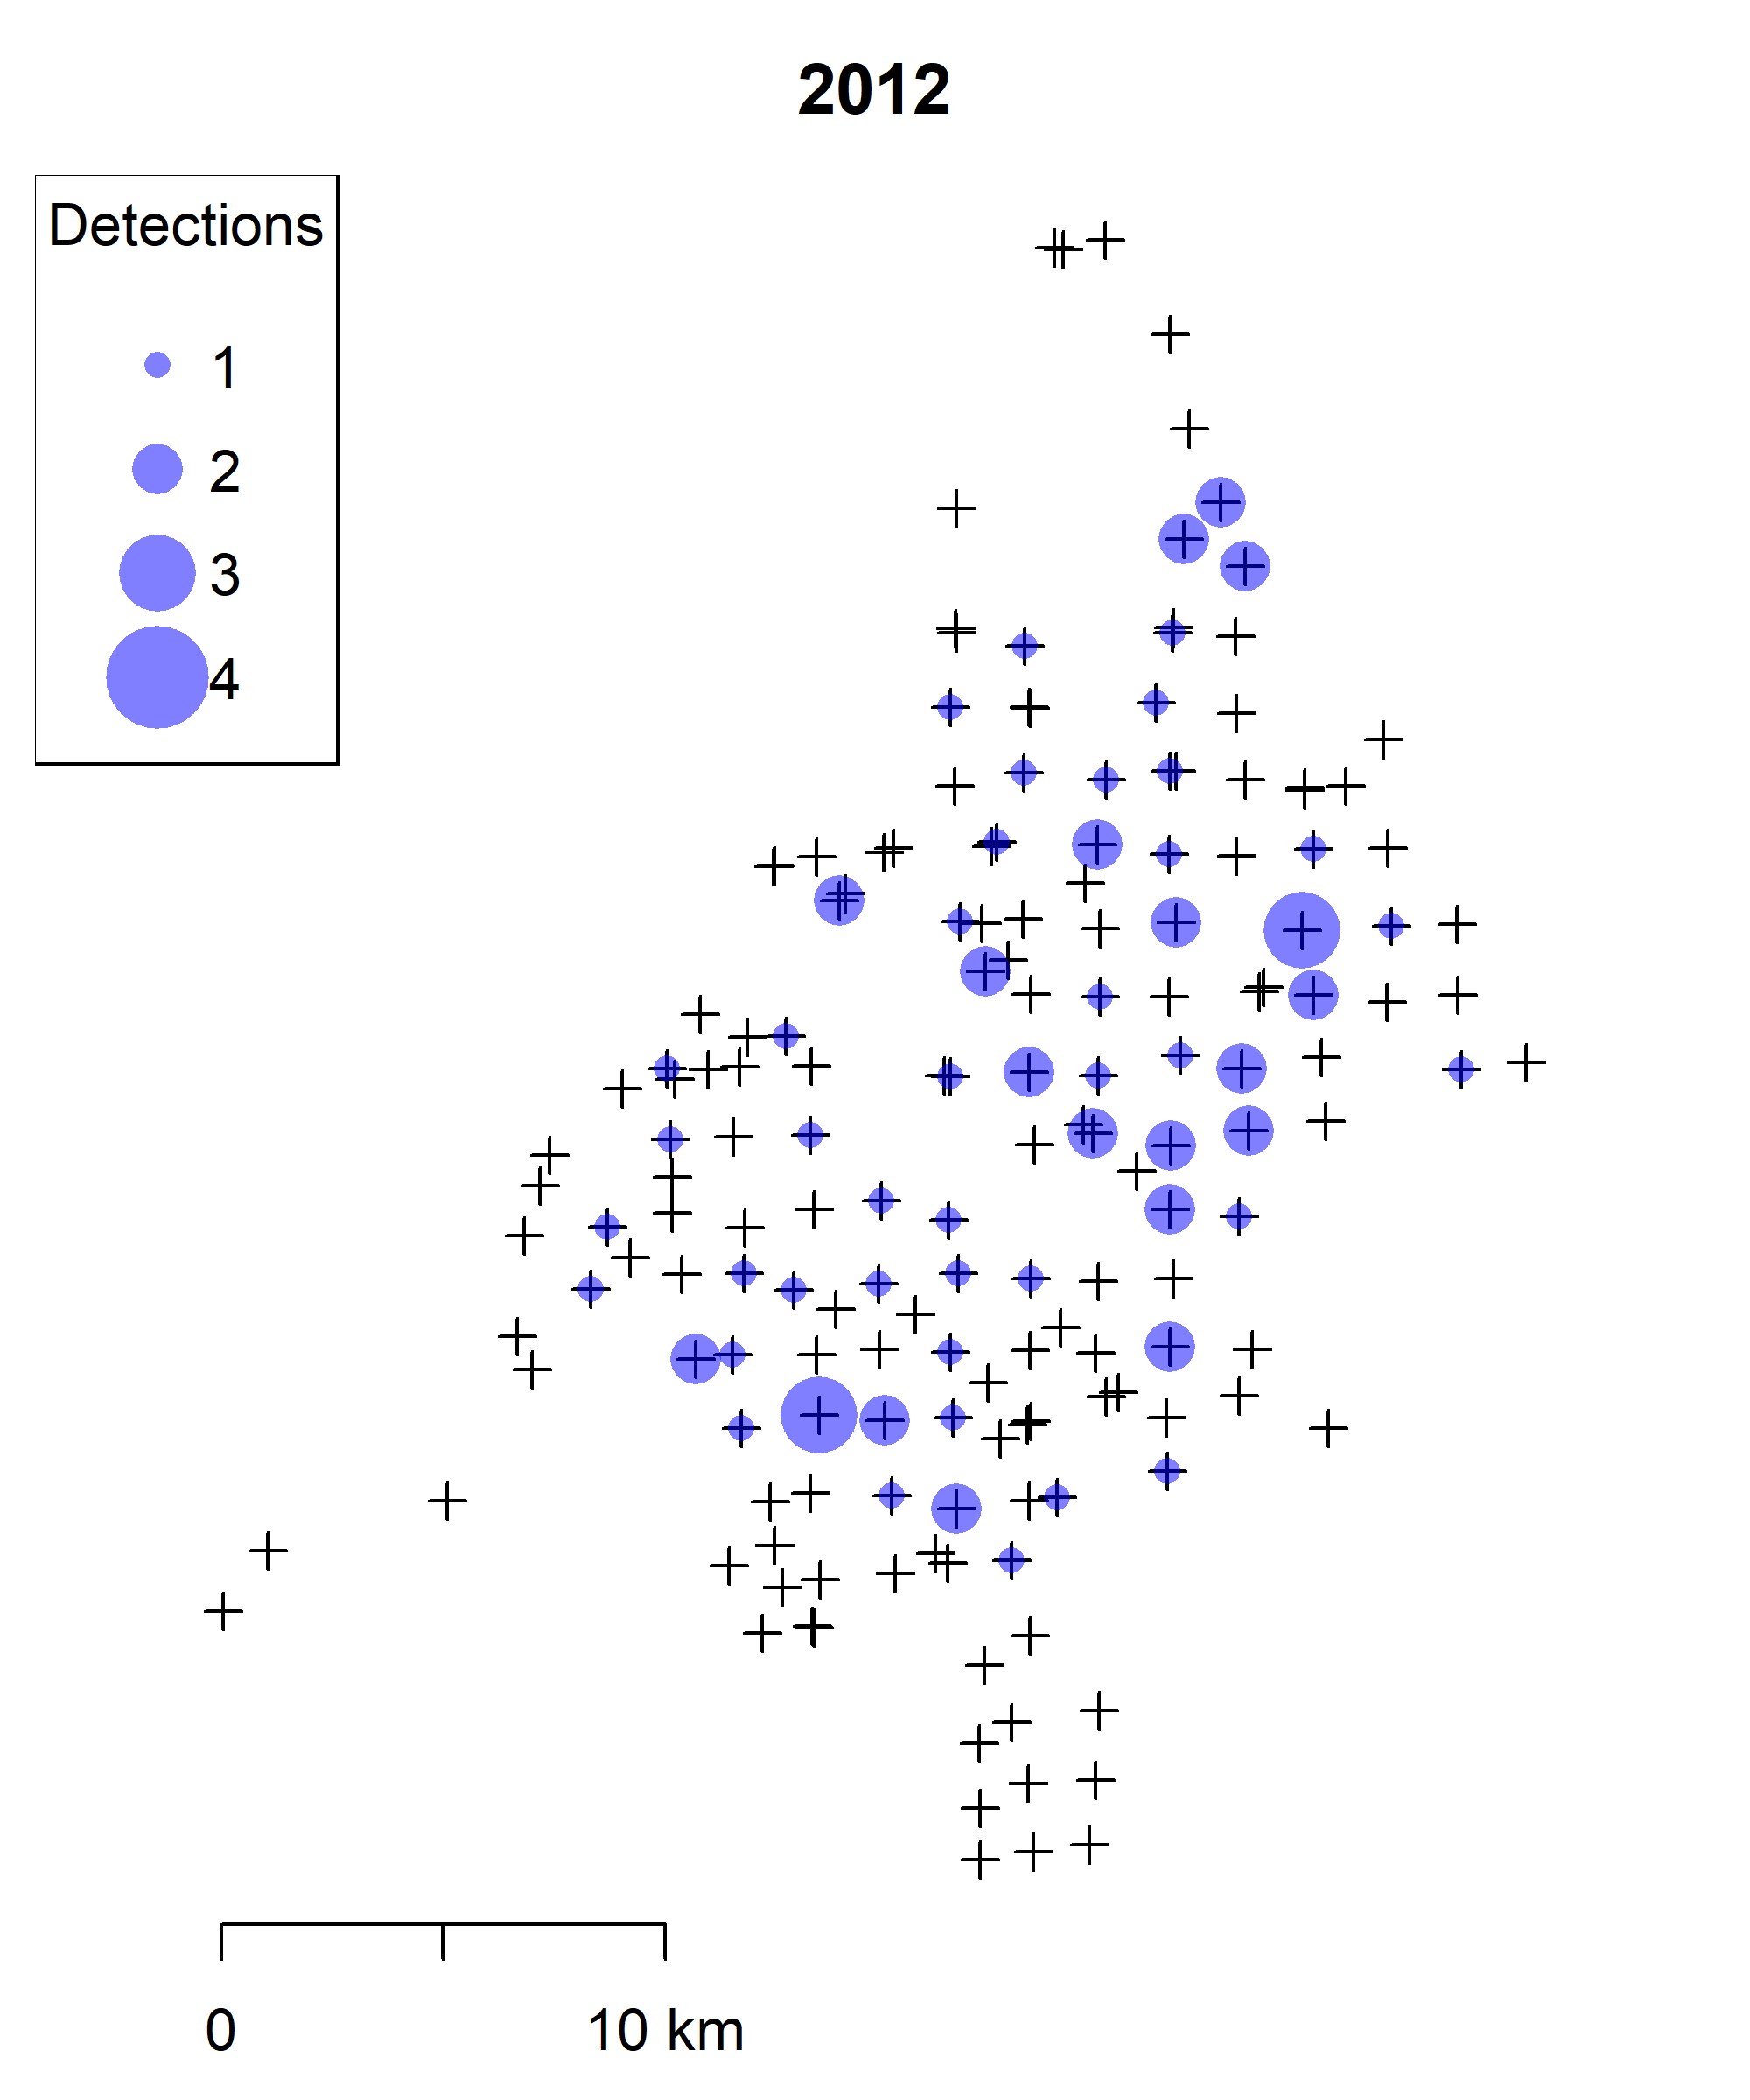
\includegraphics[width=0.3\textwidth]{figs/dets2012}} \hfill
  {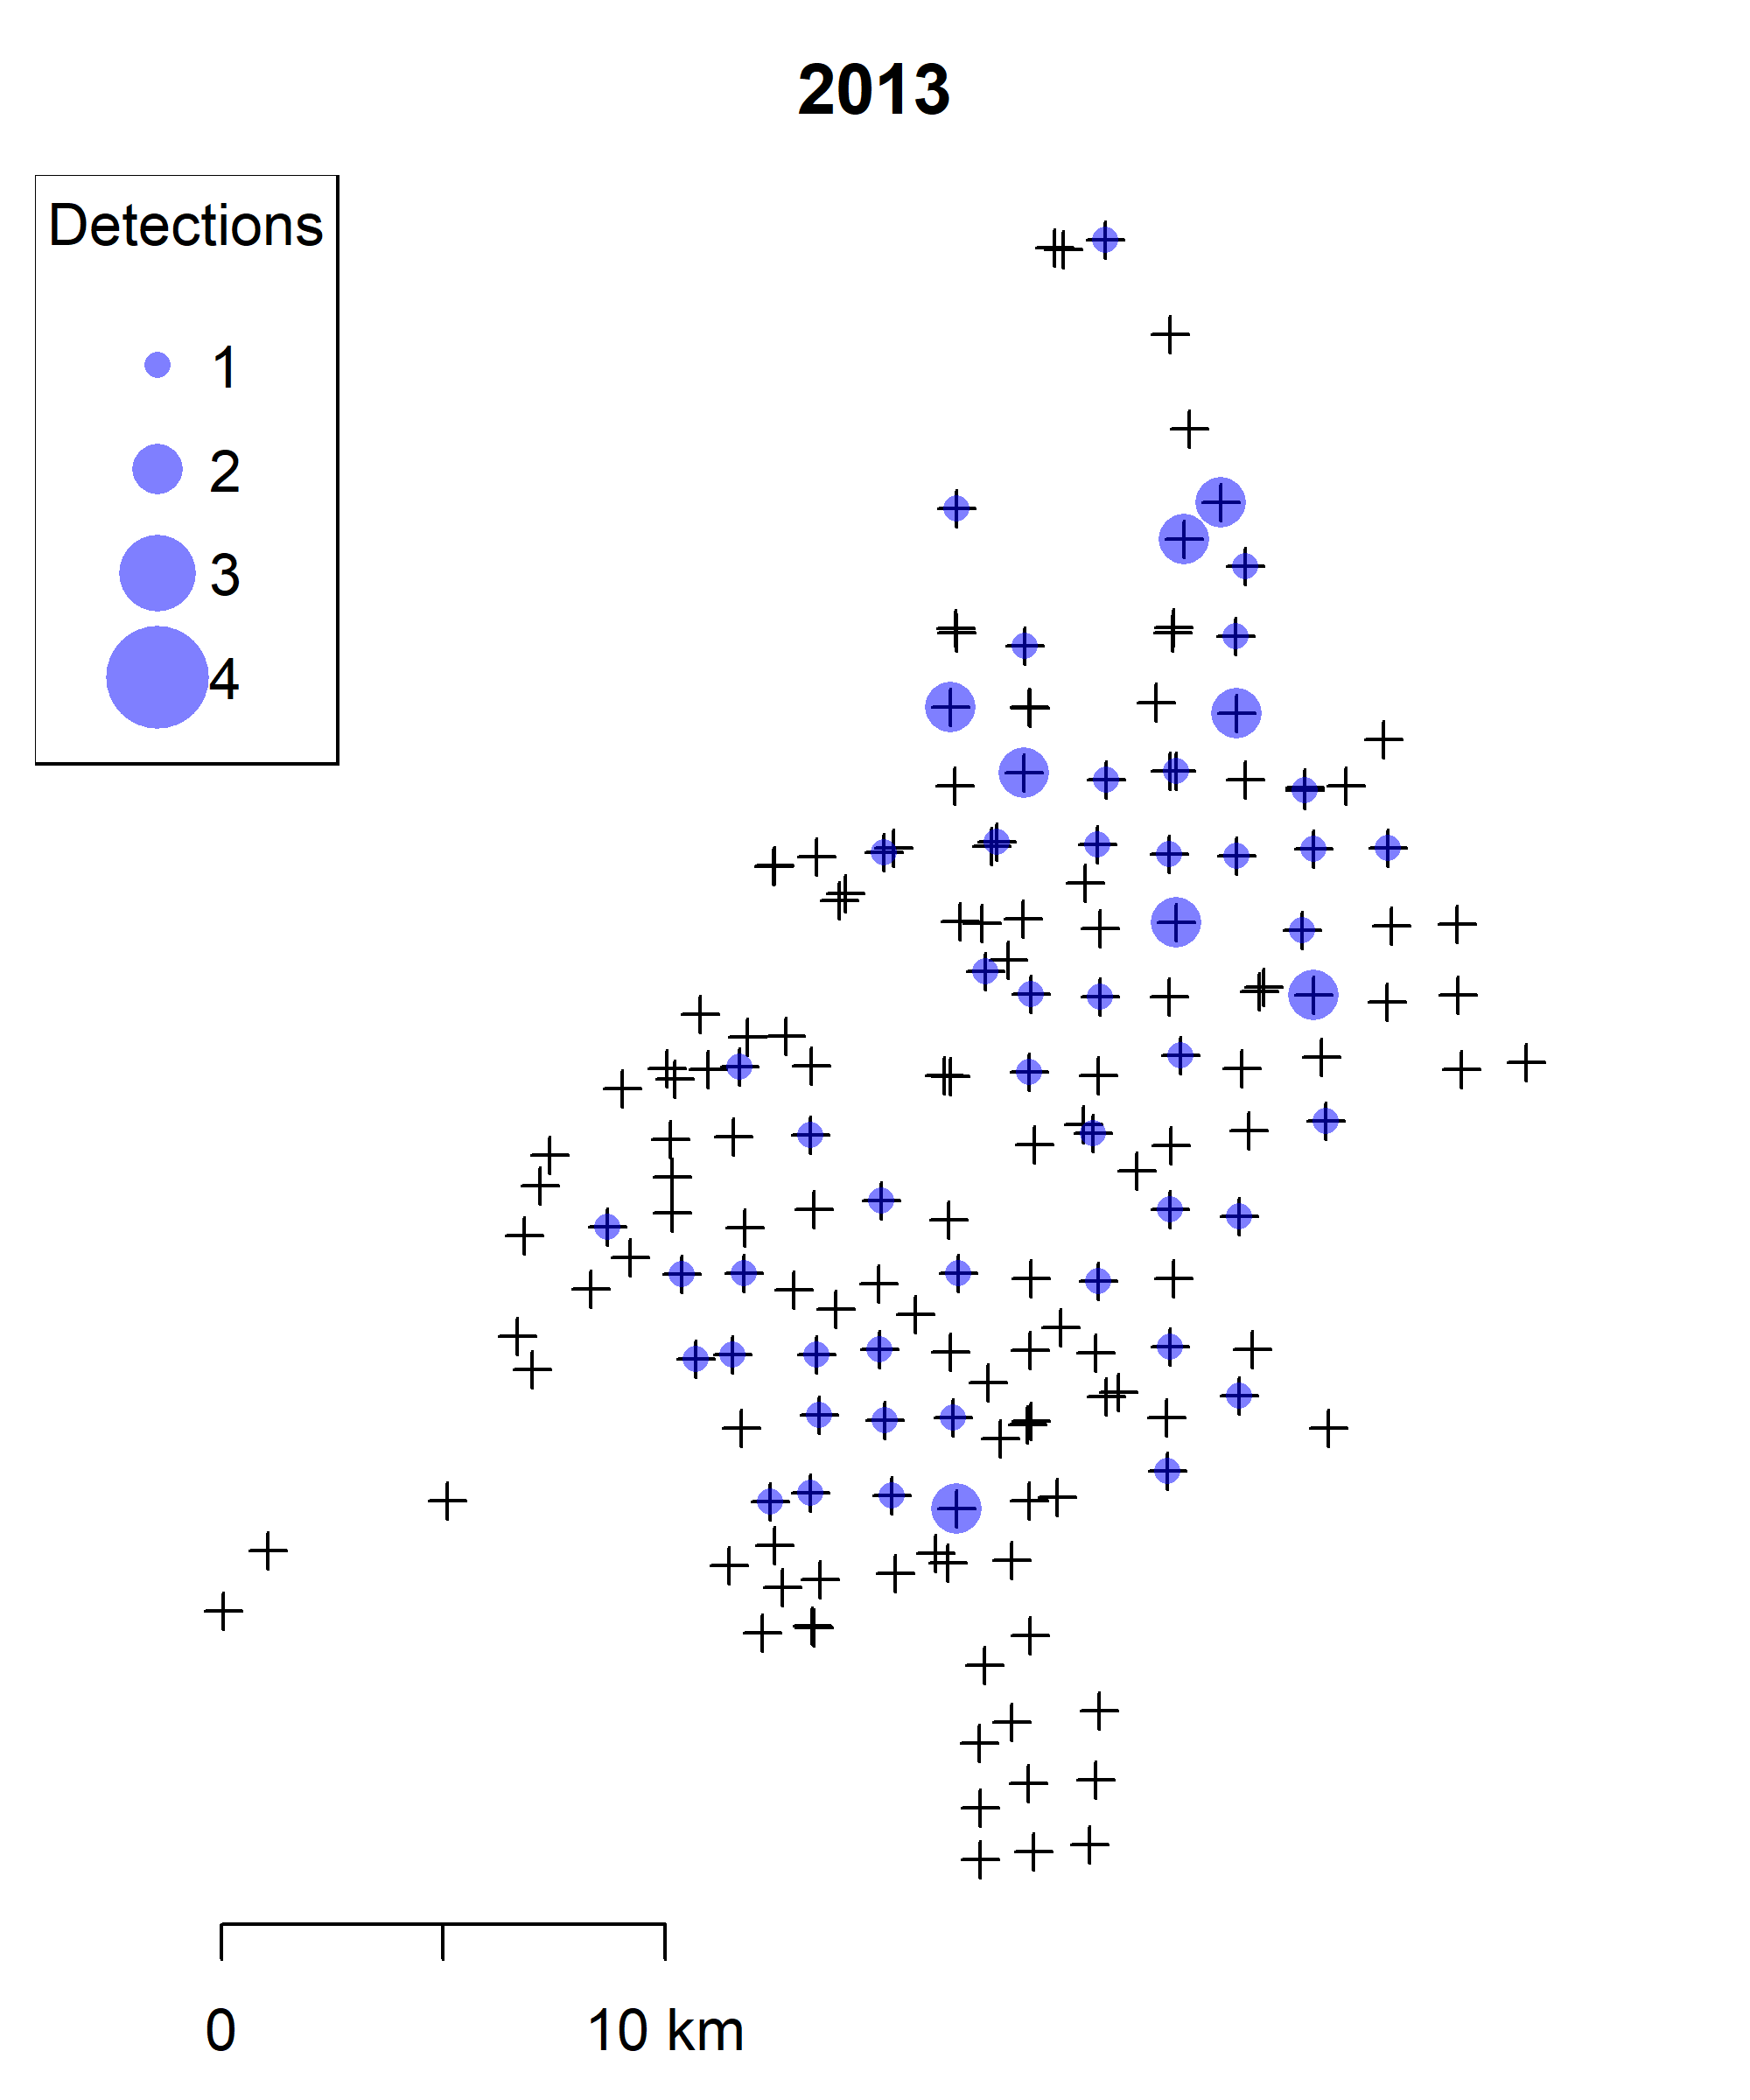
\includegraphics[width=0.3\textwidth]{figs/dets2013}} \hfill
  {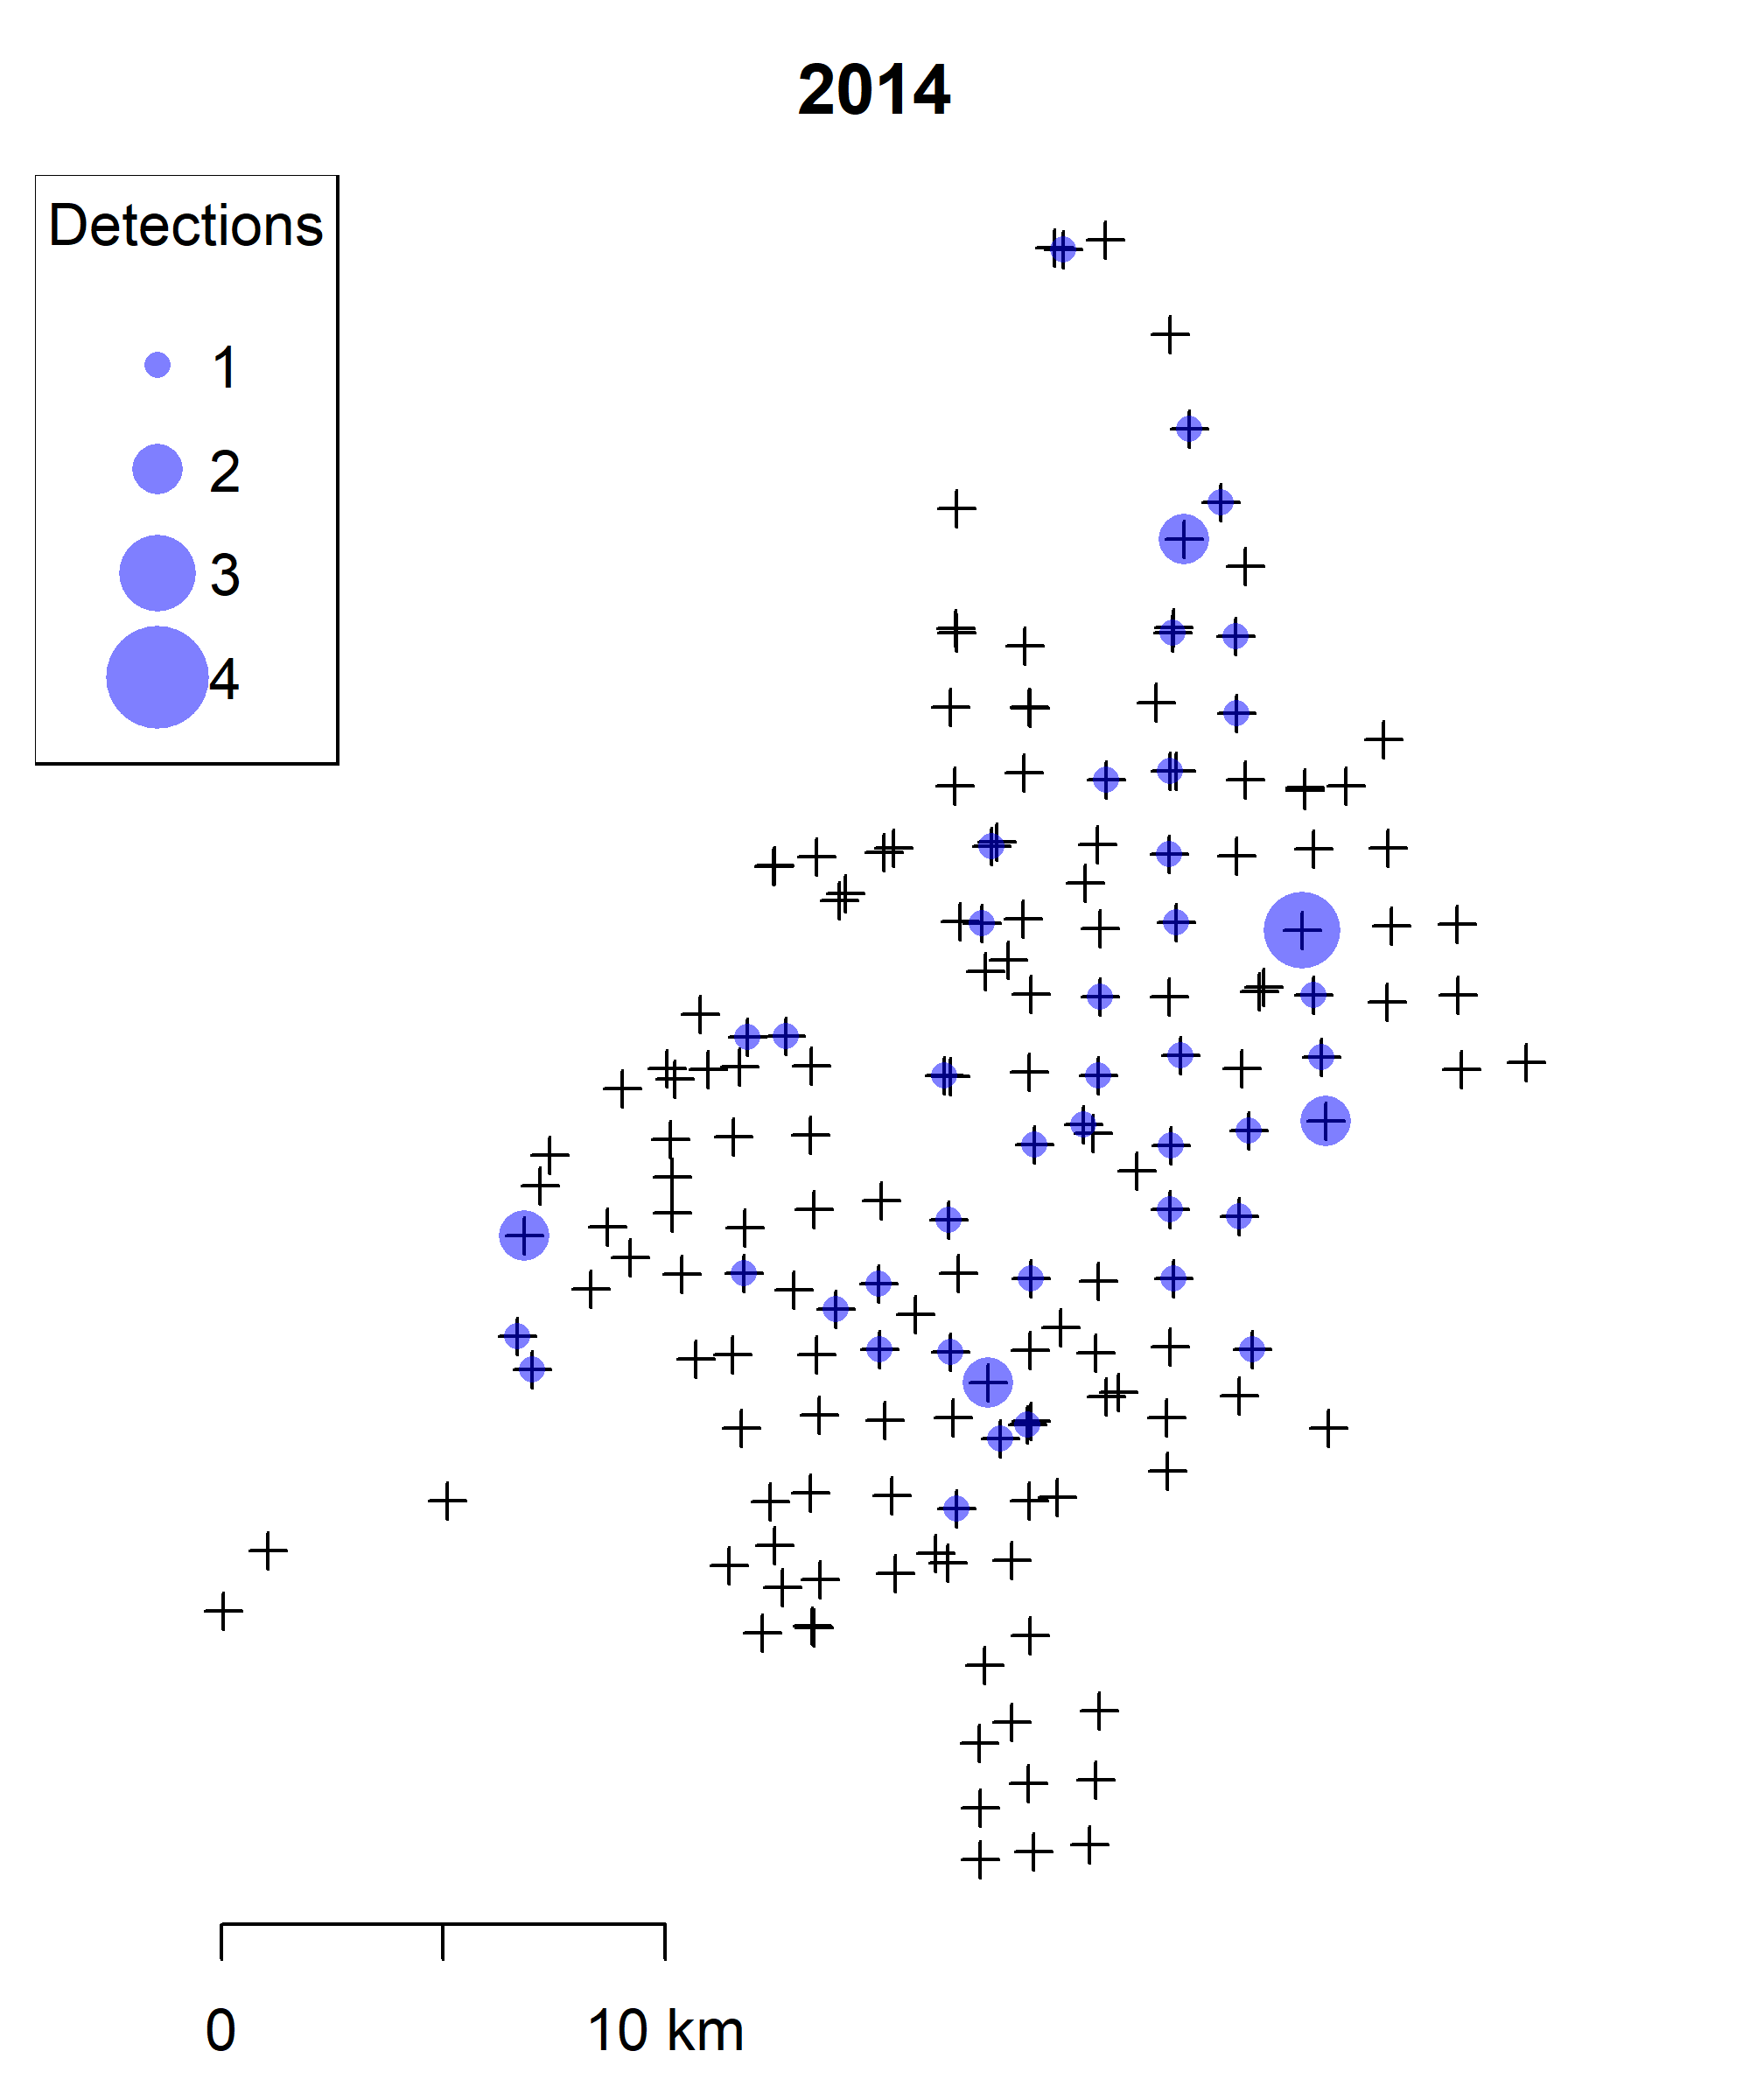
\includegraphics[width=0.3\textwidth]{figs/dets2014}} \\
  {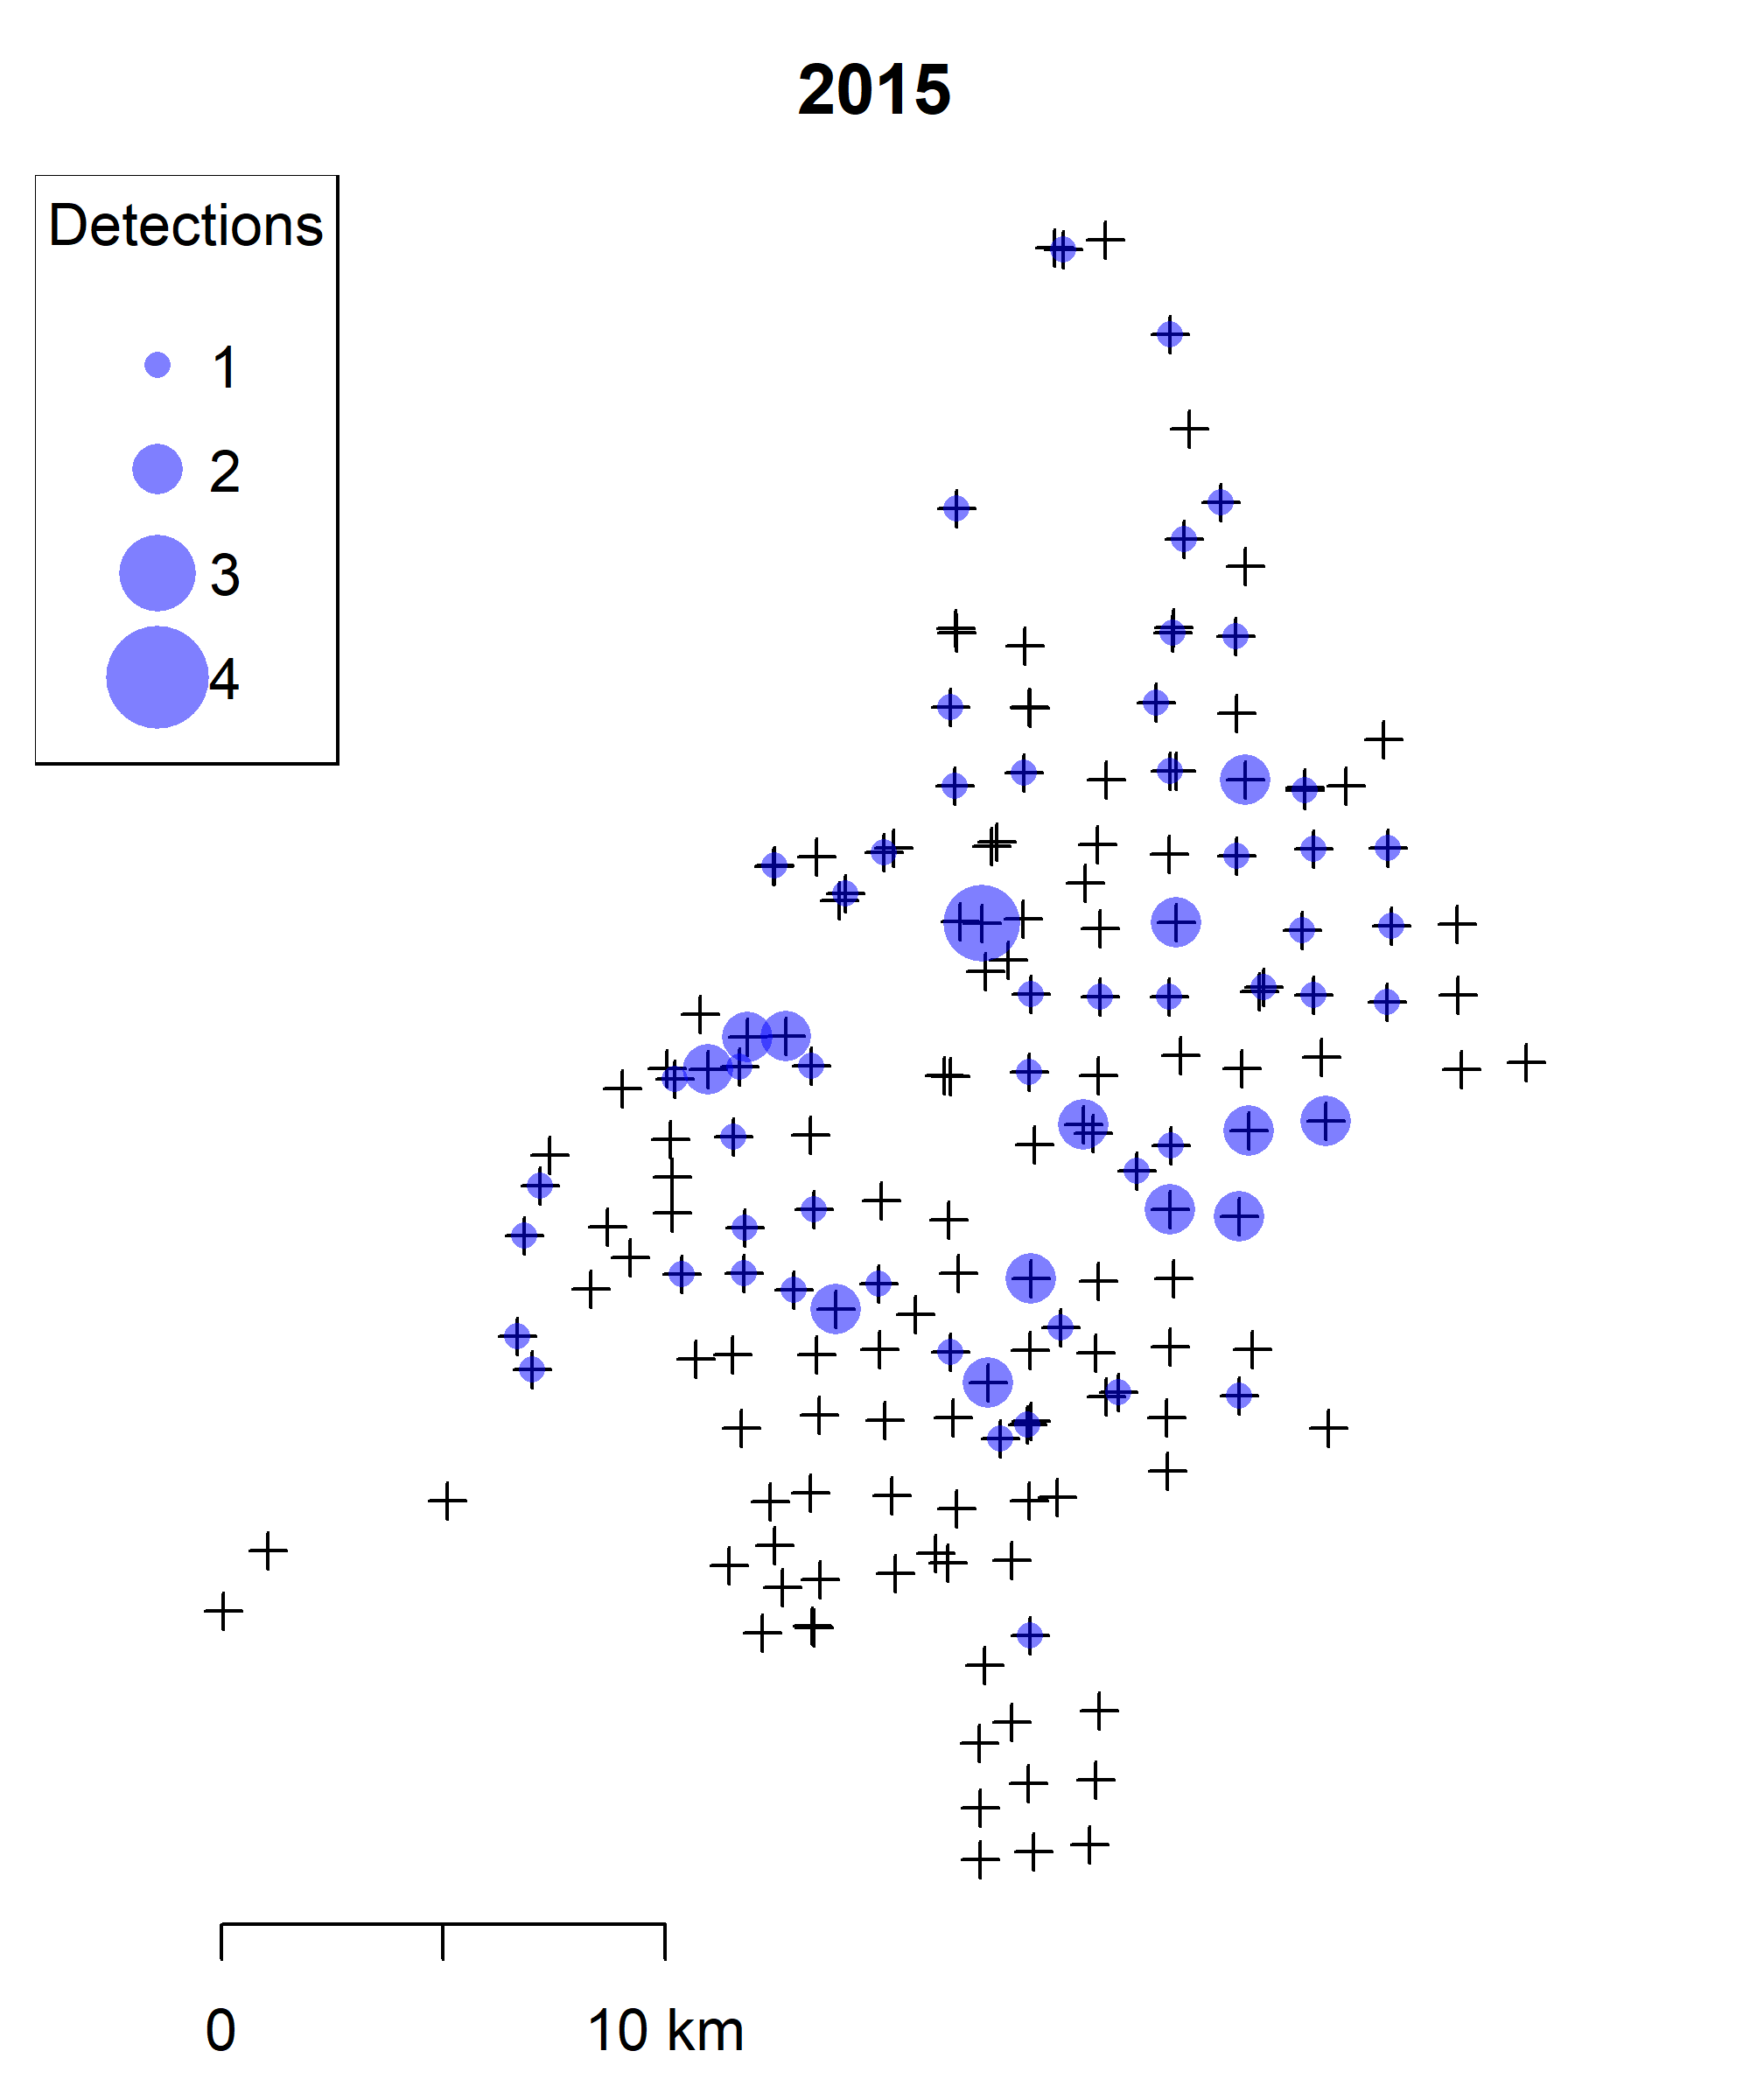
\includegraphics[width=0.3\textwidth]{figs/dets2015}} \hspace{12pt}
  {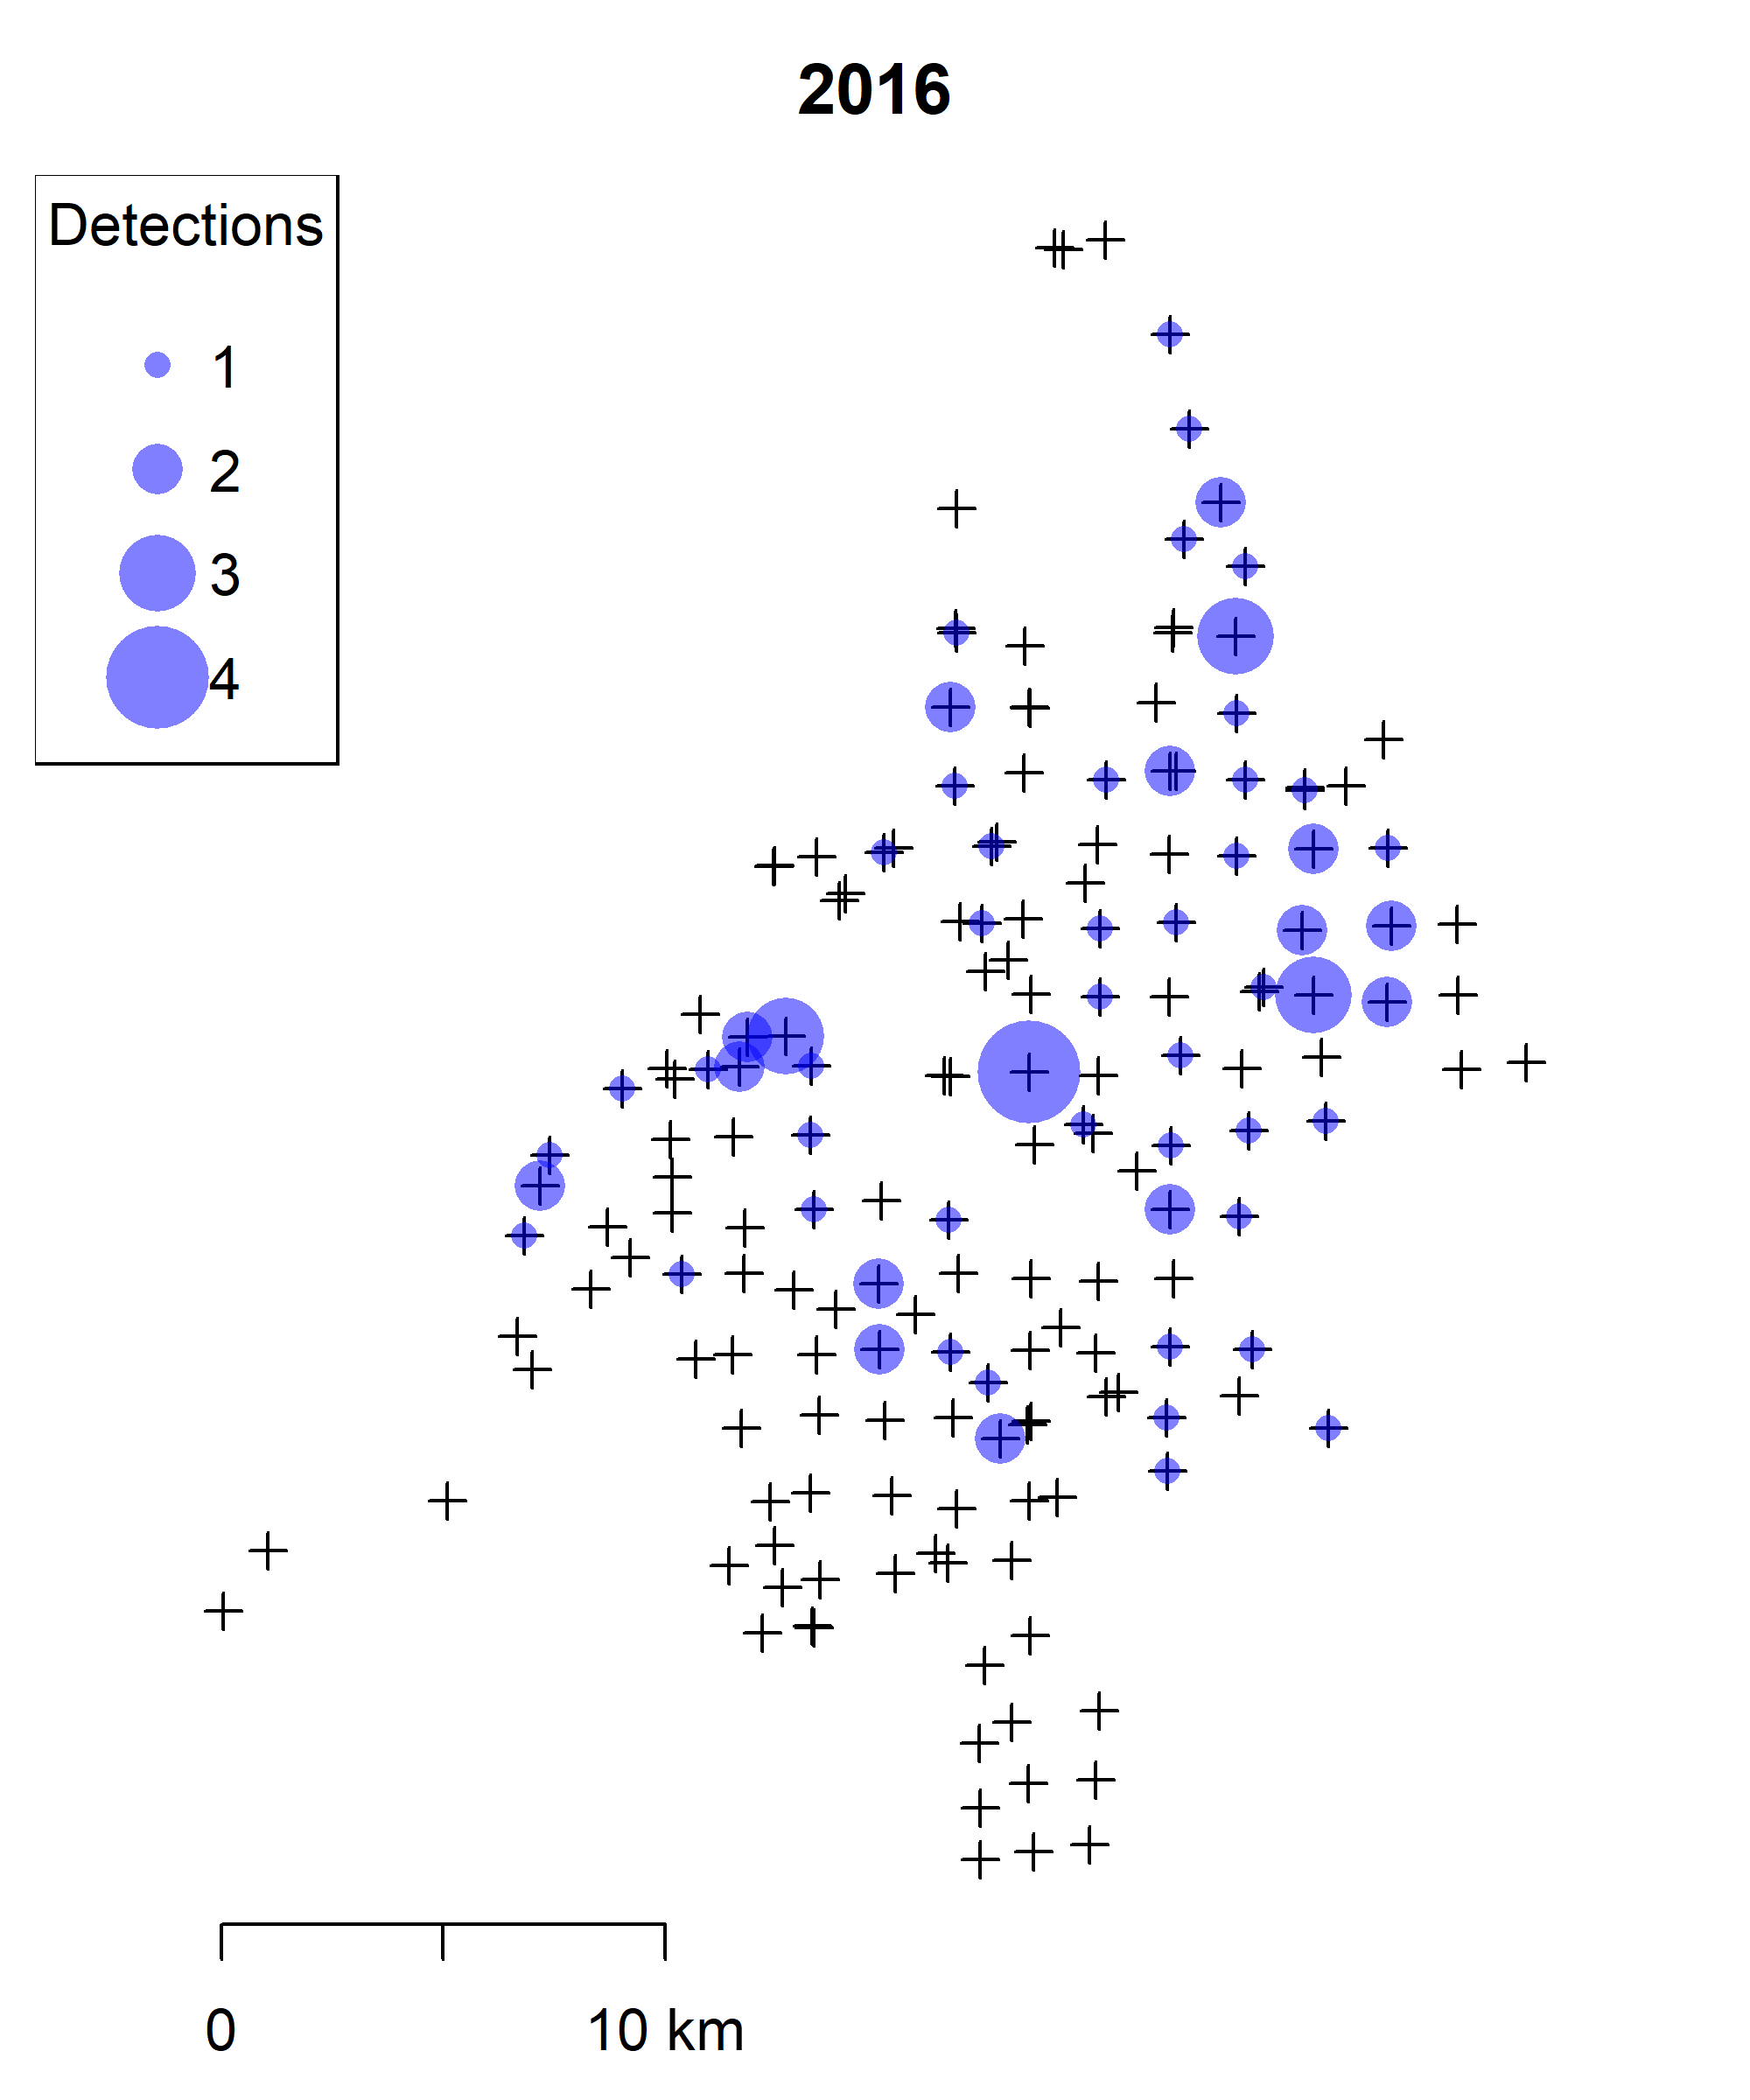
\includegraphics[width=0.3\textwidth]{figs/dets2016}} %}
  \caption{The number of female black bears detected at hair
    snares, represented by black crosses.}
  \label{fig:detmaps}
\end{figure}

\clearpage

The repository contains code for assessing the consequences of
modifying the state-space used in the spatial-capture recapture model.
The original state-space and the modified version are shown in  
Fig.~\ref{fig:2ss}. The state-space used in the manuscript was
created using landcover layers and prior information about 
space use and distribution of black bears in the Central Georgia
population. The modified state-space was similar to the original
version but the interior patches of non-habitat were included.  

\begin{figure}[h]
  \centering
  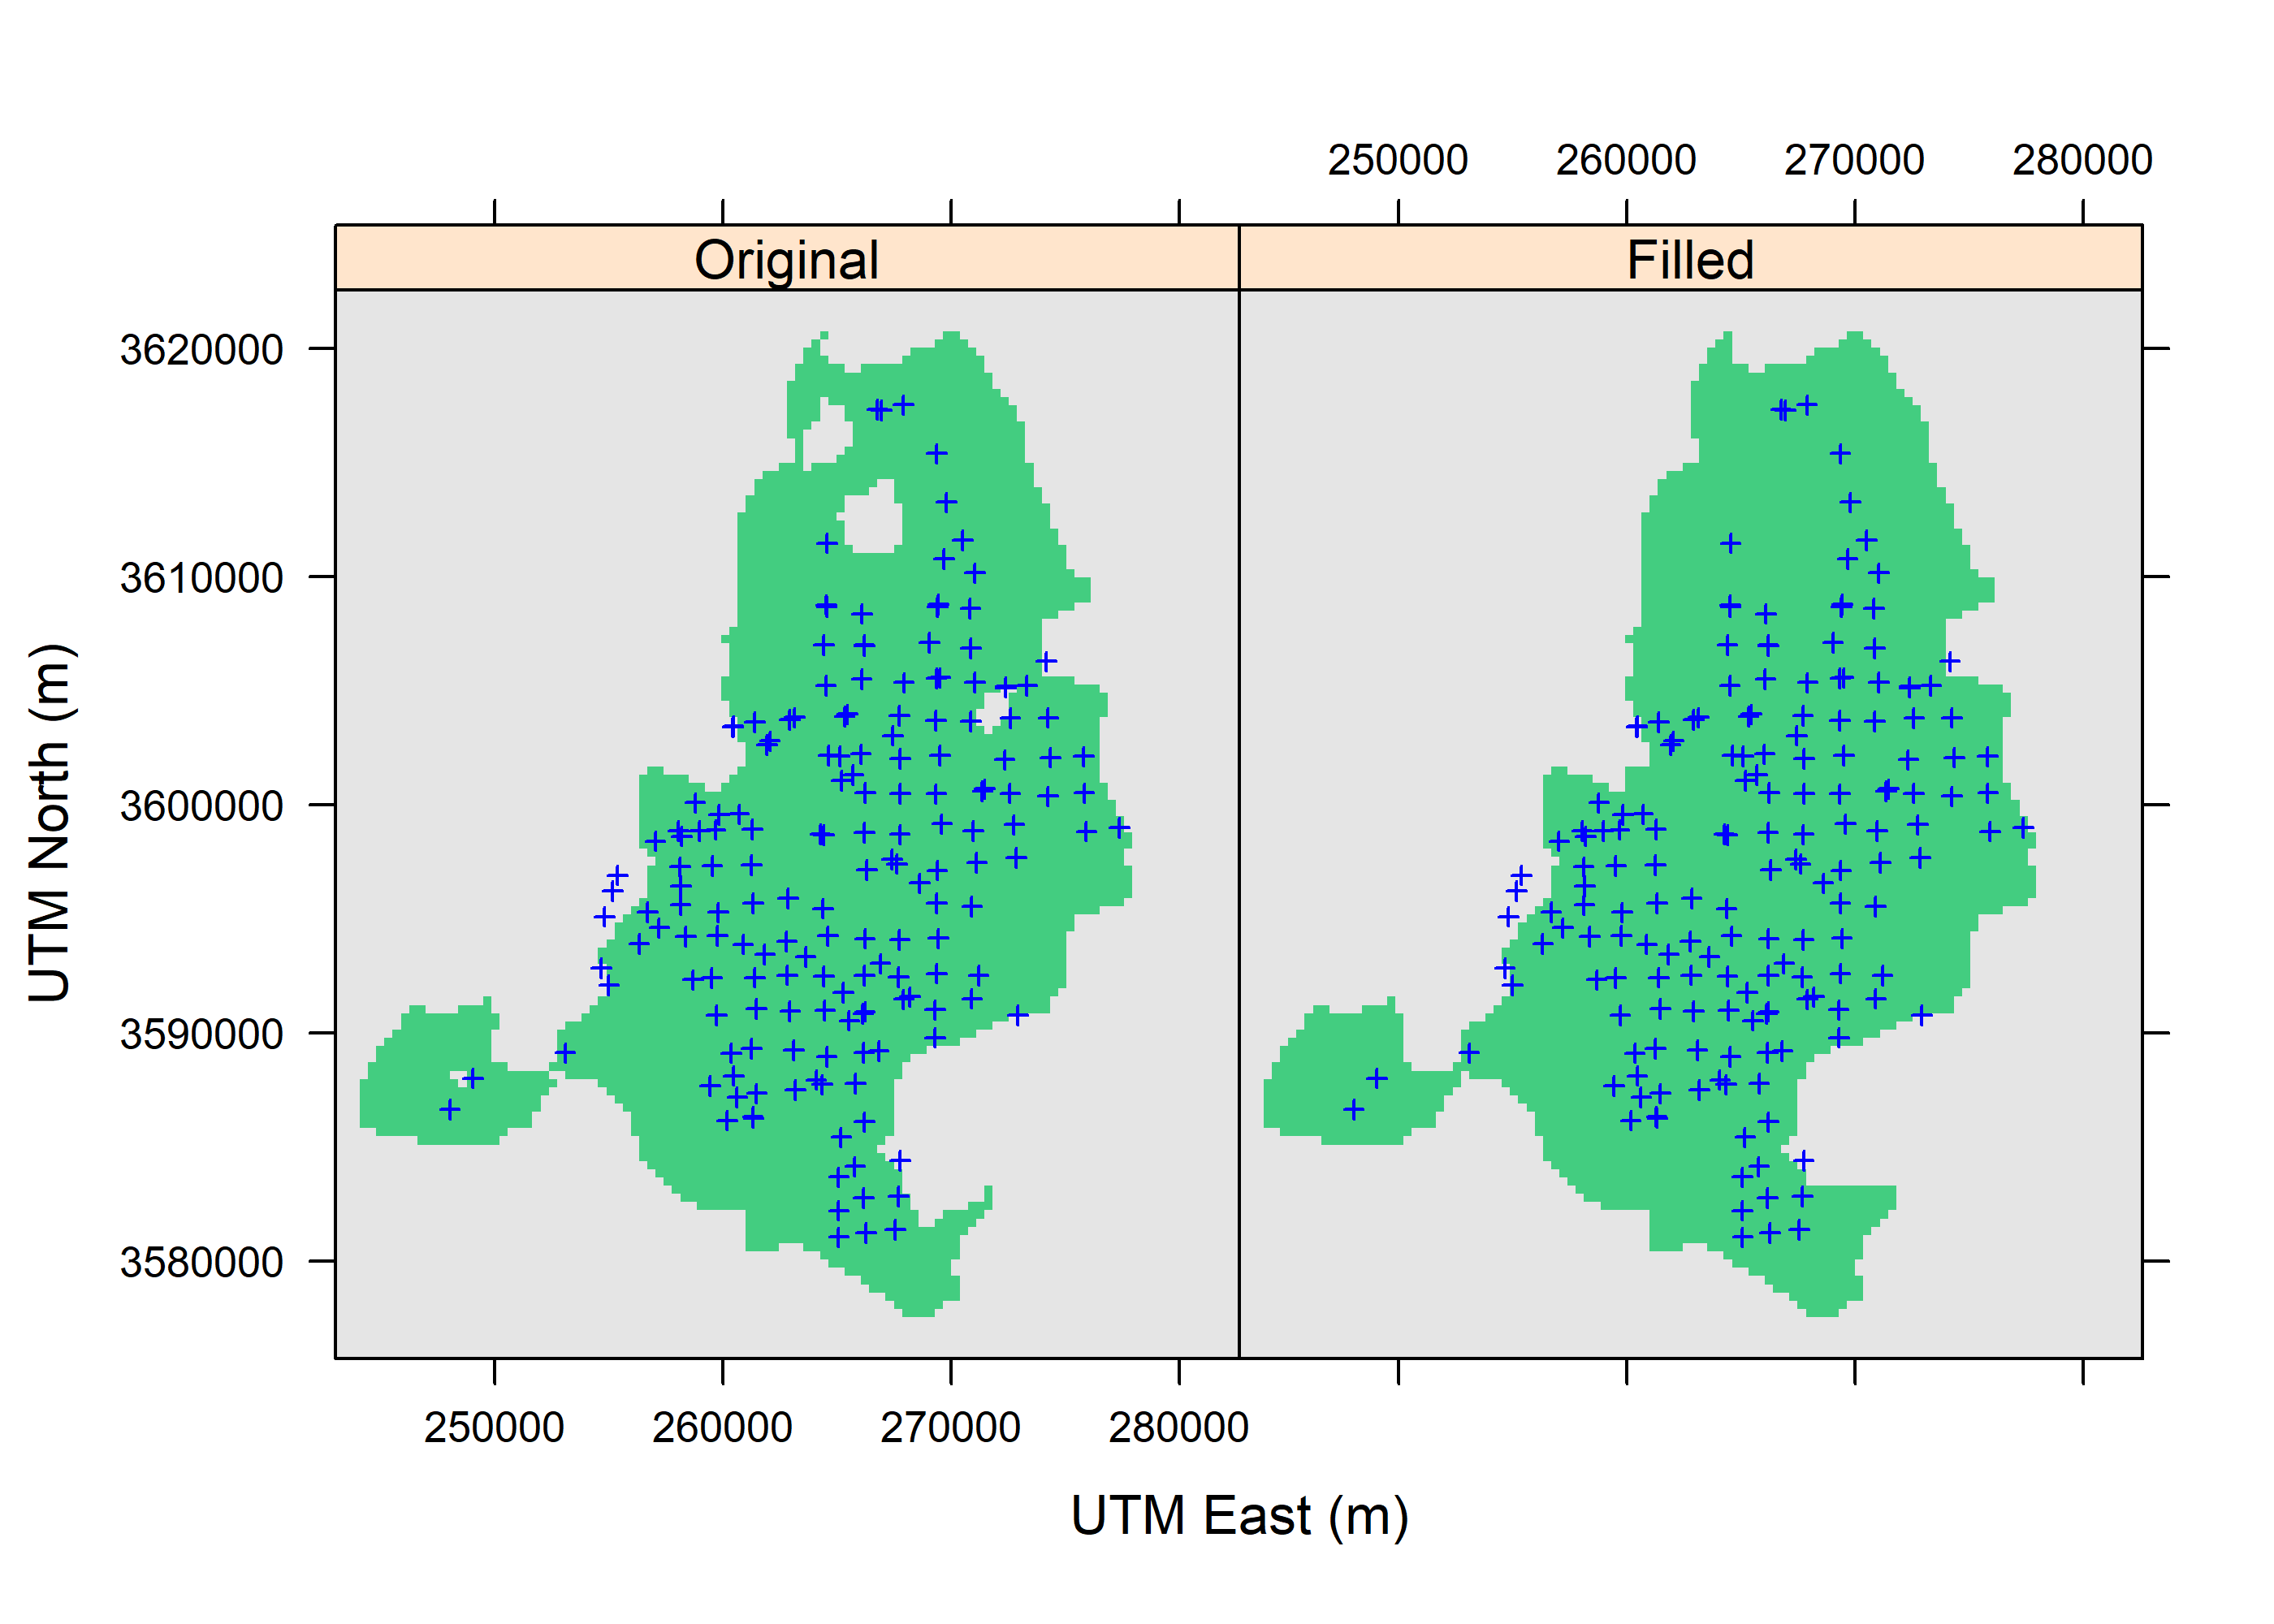
\includegraphics[width=\textwidth]{figs/state-spaces}
  \caption{The state-space on the left was created using information
    from previous research in the area. The state-space on the right
    is similar to the first, but the interior patches of non-habitat
    are filled in.}   
  \label{fig:2ss}
\end{figure}

\clearpage

%\section*{Abundance estimates}

Abundance estimates (Fig.~\ref{fig:N}) and extinction risk curves
(Fig.~\ref{fig:EX}) were similar for the two state-spaces. Abundance
estimates differed by less than five individuals each year. For both
state-space options, extinction risk was $<$1\% at year 50 when fewer
than 10 additional females were harvested each year. 


\begin{figure}[h]
  \centering
  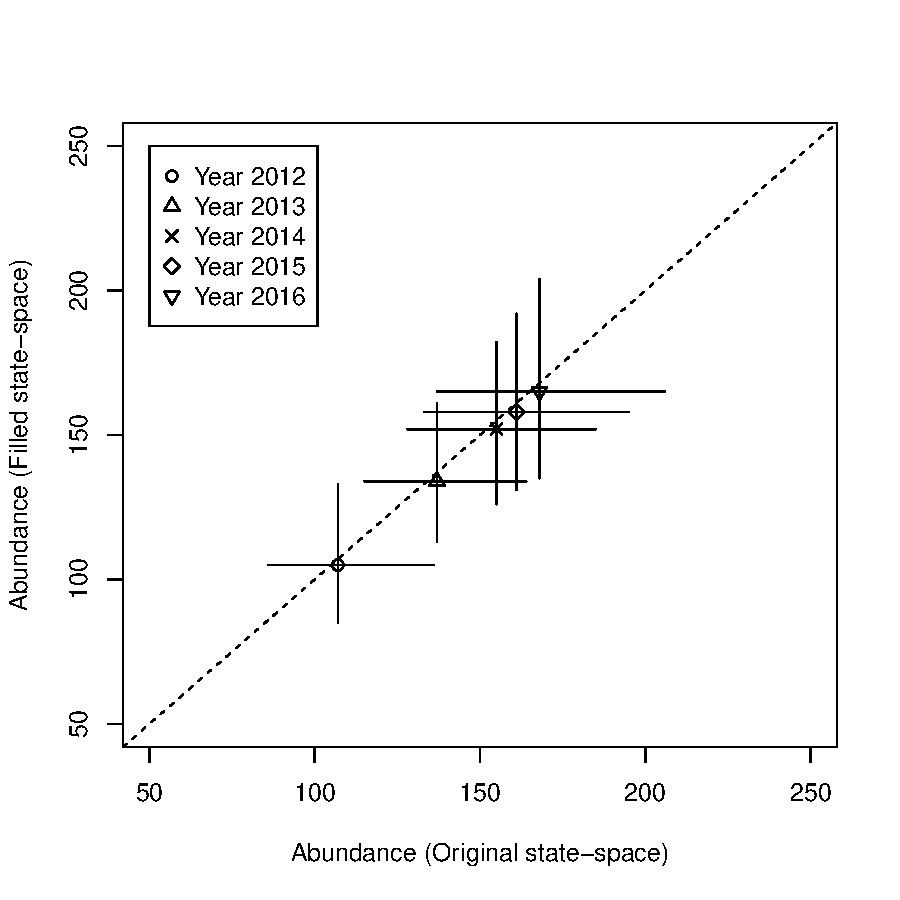
\includegraphics[width=0.8\textwidth]{figs/N_SS1vSS2} 
  \caption{Comparisons of abundance estimates in 2012--2016 using the
    two state-spaces. Error bars are 95\% credible intervals.}
  \label{fig:N}
\end{figure}

%\clearpage

%\section*{Extinction risk curves}


\begin{figure}[h]
  \centering
  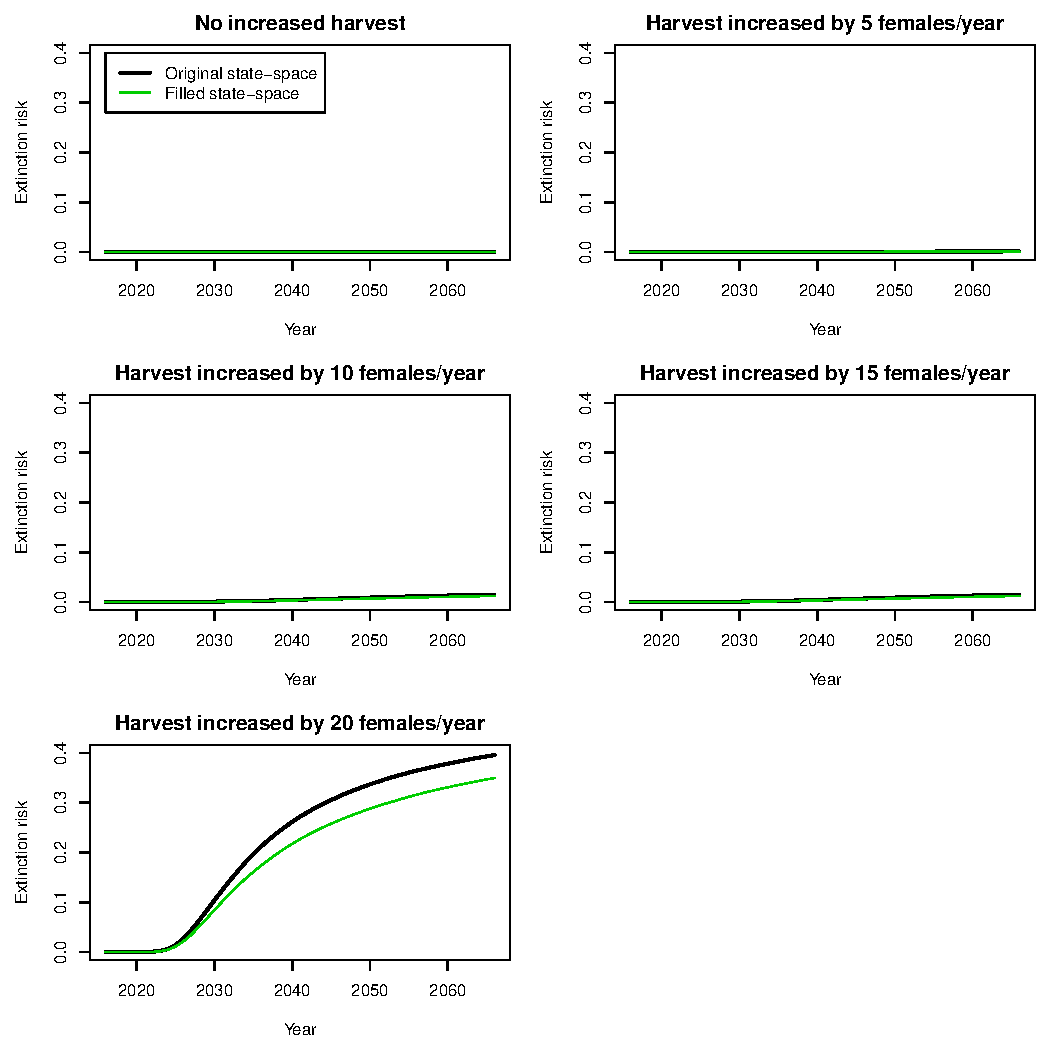
\includegraphics[width=\textwidth]{figs/EX_SS1vSS2} 
  \caption{Comparisons of extinction risk curves using the
    two specifications of the state-space.}
  \label{fig:EX}
\end{figure}




\end{document}
